\documentclass{standalone}
\usepackage{tikz}

\usetikzlibrary{calc}


\begin{document}

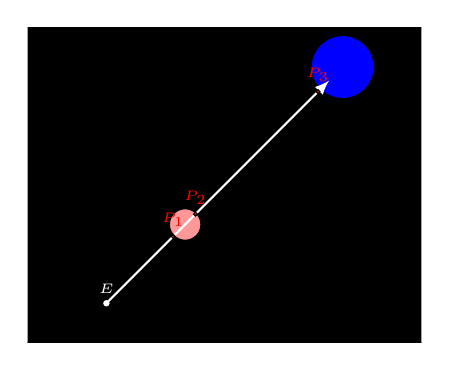
\begin{tikzpicture}
  \path[clip] (-2,0) rectangle (3,4);
  \draw[fill=black,black] (-3,0) rectangle (5,5);

  \coordinate (eye) at (-1, .5);
  \draw[fill=white] (eye) circle [radius=.05];
  \node[anchor=south,white,font=\tiny] at (eye) {$E$};

  \draw[fill=red!40] ($ (eye) + (1,1) $) circle [radius=.2];
  \draw[fill=blue] ($ (eye) + (3,3) $) circle [radius=.4];
  \draw[thick,-latex,white] (eye) -- ++(45:4);

  \coordinate (p1) at ($ (eye) + (45:1.2) $);
  \coordinate (p2) at ($ (eye) + (45:1.6) $);
  \coordinate (p3) at ($ (eye) + (45:3.8) $);
  \draw[fill=red] (p1) circle [radius=0.025] node[red,font=\tiny,above] {$P_1$};
  \draw[fill=red] (p2) circle [radius=0.025] node[red,font=\tiny,above] {$P_2$};
  \draw[fill=red] (p3) circle [radius=0.025] node[red,font=\tiny,above] {$P_3$};
\end{tikzpicture}

\end{document}